\documentclass[conference]{IEEEtran}
\usepackage{fontspec}
\setmainfont{texgyretermes}[Extension=.otf,UprightFont=*-regular,BoldFont=*-bold,ItalicFont=*-italic,BoldItalicFont=*-bolditalic]
\usepackage[spanish]{babel}
\addto\captionsspanish{\renewcommand{\tablename}{Tabla}}
\usepackage{graphicx,booktabs,amsmath,url,balance}
\usepackage[hidelinks]{hyperref}
\hypersetup{pdftitle={Comparación reproducible de CNN y YOLO26n-cls para imágenes renales},pdfauthor={Juan Fernando Jaimes Pérez y Miguel Andrés Veloza}}
\graphicspath{{../results/}{../results/full/}{figures/}}
\renewcommand{\IEEEkeywordsname}{Palabras clave}
\title{Comparación reproducible de una CNN de referencia y YOLO26n-cls para clasificación de imágenes renales}
\author{\IEEEauthorblockN{Juan Fernando Jaimes Pérez y Miguel Andrés Veloza}
\IEEEauthorblockA{Programa de Ingeniería de Sistemas\\Universidad Simón Bolívar, sede Cúcuta\\Cúcuta, Colombia}}
\begin{document}
\maketitle
\begin{abstract}
Se comparó una red convolucional de referencia publicada en Kaggle con YOLO26n-cls para clasificar imágenes renales en quiste, normal, cálculo y tumor. Se descargó la versión 2 de la recopilación de GonzaJL y se auditaron sus archivos antes de formar las particiones. De 11.756 imágenes legibles se retiraron 1.225 copias exactas adicionales. Las 10.531 imágenes restantes se distribuyeron en 7.372 de entrenamiento, 2.633 de prueba y 526 de validación, manteniendo los grupos de similitud dentro de un único conjunto. Cada arquitectura se entrenó desde cero con cinco semillas, imágenes de 224 por 224, Adam, un máximo de 20 épocas y paciencia de cinco. La selección del checkpoint se realizó mediante F1 macro de validación. En prueba, la CNN obtuvo F1 macro medio 0{,}7077 y YOLO26n-cls 0{,}7478. La diferencia media YOLO menos CNN fue 0{,}0400, con valor p bilateral exacto 0{,}1875. La latencia mediana media fue 1{,}5233 ms para la CNN y 6{,}3146 ms para YOLO. Las cinco repeticiones describen la variabilidad del entrenamiento sobre una partición fija. La interpretación del desempeño queda limitada por la procedencia heterogénea y la ausencia de identificadores verificables de paciente.
\end{abstract}

\begin{IEEEkeywords}
clasificación de imágenes, riñón, redes convolucionales, YOLO26, reproducibilidad, fuga de datos.
\end{IEEEkeywords}
\section{Introducción}
La clasificación automática de imágenes renales se ha estudiado como apoyo al análisis de quistes, cálculos y tumores. Su evaluación exige definir qué representa cada etiqueta y cómo se distribuyen las imágenes entre los conjuntos de entrenamiento y evaluación. Una exactitud elevada sobre cortes de un conjunto público requiere interpretarse en relación con su procedencia, las transformaciones aplicadas y la independencia entre ejemplos. Las decisiones aprendidas pueden depender tanto de la anatomía como de características del proceso de adquisición y almacenamiento.

La recopilación de GonzaJL disponible en Kaggle organiza imágenes en cuatro clases, Cyst, Normal, Stone y Tumor \cite{dataset}. La unidad de predicción de este trabajo es una imagen completa. La etiqueta señala la categoría asignada por el dataset. Esta formulación permite comparar una CNN convencional con una variante de clasificación de la familia YOLO. El resultado por imagen consiste en cuatro probabilidades y una categoría predicha.

El notebook público de Tahmeed \cite{baseline} ofrece una arquitectura compacta entrenada desde cero sobre esta misma recopilación. Su registro histórico permite identificar capas e hiperparámetros, pero usa una división de entrenamiento y validación distinta de la adoptada en este estudio. Reproducir la arquitectura y explicar los cambios de protocolo permite evaluar su comportamiento bajo una partición común y documentada.

YOLO surgió como una familia de detectores de una sola etapa \cite{yolo}. Las implementaciones de Ultralytics incluyen variantes específicas de clasificación. YOLO26n-cls reutiliza un backbone convolucional y la cabeza Classify \cite{yolo26,ultralytics}. El interés de la comparación es medir el desempeño y costo de ambas redes con imágenes, semillas y presupuesto compartidos. Las cifras publicadas en otros conjuntos sirven como antecedentes para formular el estudio.

El objetivo es comparar la CNN de referencia y YOLO26n-cls mediante cinco entrenamientos independientes por modelo, usando F1 macro como métrica principal. Se evalúan además exactitud, precisión, recall, desempeño por clase, tiempo de entrenamiento y latencia. La contribución práctica es un experimento verificable que incorpora auditoría de duplicados, agrupamiento de similitudes, un manifiesto compartido y conservación de predicciones por ejecución.
El código y los resultados del experimento se conservan en el repositorio del proyecto\footnote{\url{https://github.com/juanfernandojaimesperez63-source/comparacion-renal-cnn-yolo-publico}}, de acceso público.
\section{Trabajos relacionados}
Islam y colaboradores \cite{islam} describieron el conjunto de TC renal de hospitales de Dhaka y estudiaron redes de transferencia y Vision Transformers. Esta fuente ayuda a identificar una parte de la procedencia declarada de la recopilación de GonzaJL. La recopilación empleada aquí agrega otras fuentes, por lo que la correspondencia entre ambos conjuntos debe verificarse por archivos y metadatos.

Pande y Agarwal \cite{pande} estudiaron YOLOv8n-cls en imágenes renales del conjunto original de 12.446 imágenes. Su trabajo constituye un antecedente directo de clasificación renal con una variante YOLO. Su división 80/20 y la terminología de detección usada en partes del artículo requieren cautela al interpretar sus figuras y métricas junto a un experimento de clasificación con prueba independiente.

KidneyNet \cite{kidneynet} propone una CNN para diagnóstico automático a partir de TC y muestra el interés de desarrollar arquitecturas específicas para el problema renal. LiteRenalNet \cite{lite} combina ramas de detalle y semántica con atención espacial y por canales. Estos trabajos motivan evaluar conjuntamente capacidad predictiva, complejidad e interpretación, aunque sus arquitecturas y protocolos difieren del presente estudio. La comparación directa se limita a las dos implementaciones entrenadas aquí.

El preprint de YOLO26 \cite{yolo26} describe las variantes de clasificación y presenta un análisis de optimizadores en ImageNet en su suplemento. La cabeza Classify tiene una función documentada en código versionado \cite{ultralytics}. Este experimento utiliza Adam para ambas redes, y por ello su entrenamiento responde al protocolo compartido descrito en la sección de métodos.

\section{Materiales y métodos}
\subsection{Procedencia y auditoría de las imágenes}
Se descargó la versión 2 de la recopilación de GonzaJL. La descripción de Kaggle atribuye las imágenes a cuatro fuentes, CT Kidney Dataset, Kidney Stones MRI and CT scans, KidneyStone y Medical Scan Classification Dataset. El ZIP se identificó mediante SHA-256 y se conservaron metadatos de la consulta. La auditoría decodificó cada imagen con Pillow, registró dimensiones, modo, formato y dos hashes, uno de los bytes y otro de los píxeles RGB con sus dimensiones.

Se encontraron 11.756 imágenes válidas, 2.939 por clase. Todas tenían 224 por 224 píxeles y tres canales RGB. Se observaron 9.417 archivos JPEG y 2.339 PNG, sin errores de decodificación. El archivo datos.csv contenía 11.756 rutas distintas y las etiquetas coincidían con las carpetas. El formato presenta asociación con la clase, con todos los quistes y tumores en JPEG y parte de las clases Normal y Stone en PNG. Esta distribución debe considerarse en el análisis de posibles atajos visuales.

Kaggle declara CC0 para la recopilación. Las fuentes declaradas muestran términos heterogéneos, CC BY 4.0 para CT Kidney Dataset, licencia desconocida para dos fuentes y otros términos para Medical Scan Classification Dataset. Se conserva esta distinción en la documentación del proyecto. La procedencia y modalidad por imagen quedan sin resolver en los metadatos distribuidos, lo que limita la caracterización de subgrupos y la interpretación de la generalización entre fuentes.

\subsection{Duplicados y similitud antes de la partición}
Se identificaron 1.225 copias exactas adicionales, organizadas en 1.222 grupos con multiplicidad. En esta versión, el conteo coincidió con la comparación de bytes y de píxeles. Se conservó un representante determinista de cada conjunto idéntico. El balance original cambió al retirar 255 copias de Cyst, 172 de Normal y 798 de Stone. No se encontraron copias adicionales en Tumor.

Para imágenes de píxeles distintos se calculó un dHash de 64 bits sobre una imagen gris de 9 por 8. Se exigió distancia de Hamming de hasta cuatro bits y error cuadrático medio raíz de hasta 0,035 entre miniaturas grises de 32 por 32 normalizadas a [0,1]. El filtro combina una comparación de variaciones locales y una comprobación de intensidad global. Los umbrales se fijaron durante la preparación de los datos, antes del entrenamiento completo y de consultar las métricas de prueba.

El procedimiento identificó 21.106 pares con píxeles distintos que cumplen ambos umbrales, sin cruces de clase. Se revisó visualmente una muestra de 12 pares cerca del umbral de intensidad. Los pares se conectaron mediante componentes conexos. Una cadena de vecinos conserva a todas las imágenes de su componente dentro de una sola partición. El mayor grupo tenía 225 archivos. Este criterio puede agrupar cortes relacionados y también introducir agrupaciones conservadoras entre imágenes de aspecto similar.

La similitud visual carece de identificadores clínicos que permitan demostrar identidad de paciente. Los nombres secuenciales, el CSV y la ausencia de etiquetas EXIF útiles impiden una partición verificable por paciente. En consecuencia, la evaluación se interpreta como clasificación de imágenes con control heurístico de similitud. Queda posible una relación entre cortes de un mismo estudio que el criterio empleado no reconozca, especialmente al variar plano o apariencia.

\begin{table}[t]
\caption{Partición compartida después de eliminar copias exactas.}
\label{tab:split}\centering
\begin{tabular}{lrrrr}\toprule
Clase & Entrena & Prueba & Valida & Retira\\\midrule
Cyst & 1879 & 671 & 134 & 255\\
Normal & 1937 & 692 & 138 & 172\\
Stone & 1499 & 535 & 107 & 798\\
Tumor & 2057 & 735 & 147 & 0\\\midrule
Total & 7372 & 2633 & 526 & 1225\\\bottomrule
\end{tabular}
\end{table}
\subsection{Construcción de una partición única}
Se asignaron grupos completos con semilla de partición 27 y un objetivo estratificado de 70\% entrenamiento, 25\% prueba y 5\% validación. Este orden corresponde a la guía de la actividad. La asignación equilibró los tamaños por clase preservando la integridad de los grupos. La Tabla~\ref{tab:split} muestra los conteos finales sobre 10.531 imágenes únicas. Las fracciones resultantes fueron 70,0028\%, 25,0024\% y 4,9948\%, respectivamente.

Se guardó un único manifiesto con ruta, clase, hashes, grupo y partición. Ambos modelos consultaron ese archivo. Se verificó que ningún grupo ni hash de píxeles apareciera en más de un conjunto activo. Las copias retiradas quedaron identificadas en el mismo manifiesto para permitir inspección y reproducción. La exclusión de duplicados explica que el número de imágenes por clase deje de ser idéntico.

\begin{figure}[t]
\centering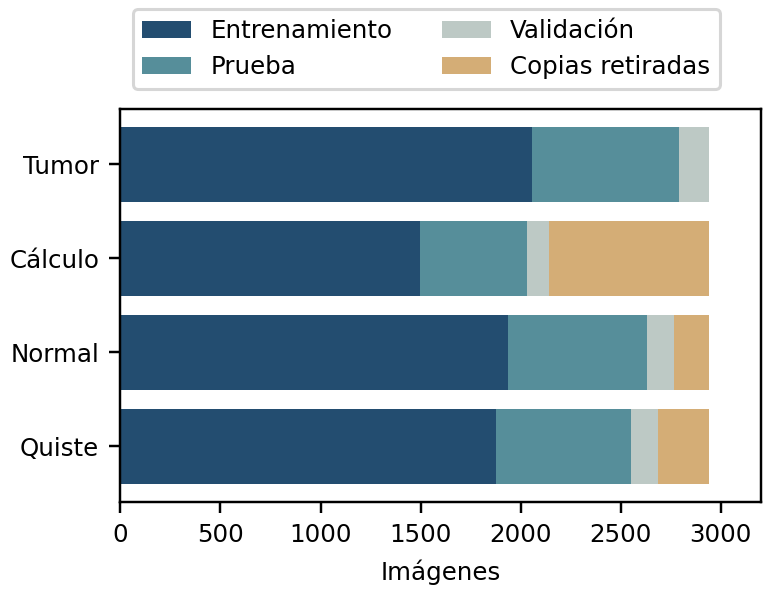
\includegraphics[width=\columnwidth]{dataset_split.png}
\caption{Distribución de la partición compartida y copias exactas retiradas.}\label{fig:split}
\end{figure}
La Fig.~\ref{fig:split} muestra el cambio de balance al retirar copias exactas. La clase Stone pierde una fracción mayor de archivos.
\subsection{CNN de referencia y fidelidad de la adaptación}
La arquitectura se tomó del notebook de Tahmeed \cite{baseline}. Consta de cuatro convoluciones con 32, 64, 128 y 256 filtros, núcleos de 5, 5, 3 y 3, stride 2, padding same y activación ReLU. Cada convolución va seguida de MaxPool de 2 por 2. La salida se aplana y pasa por una capa densa de 128 unidades con activación lineal y una capa softmax de cuatro unidades. Se verificaron 456.132 parámetros entrenables.

La arquitectura original de Keras se adaptó a PyTorch para ejecutar ambos modelos con el mismo backend en una GPU NVIDIA Tesla T4 asignada por Google Colab. Se implementó padding explícito para reproducir las dimensiones de same. Una comprobación con pesos transferidos verificó igual número de parámetros y una diferencia máxima de $4{,}47\times10^{-8}$ entre probabilidades de inferencia en tres entradas de prueba numérica. Esta comprobación valida la transformación de la arquitectura; las inicializaciones y las trayectorias de optimización pueden variar entre frameworks.

Se mantuvo la capa densa lineal observada en el código original. Los píxeles se normalizaron mediante un factor 1/255. El notebook histórico usó lotes de 64, un 25\% de validación y guardado por exactitud de validación. Este experimento usa lote 32 y selección por F1 macro de validación. Los cambios permiten alinear el protocolo entre redes y se declaran al contrastar con la cifra histórica de 0,87411 de exactitud de validación del mejor checkpoint registrado.

\subsection{YOLO26n en modo clasificación}
Se construyó el modelo desde yolo26n-cls.yaml del paquete Ultralytics 8.4.0 y se configuró nc=4. El backbone incluye convoluciones, bloques C3k2 y C2PSA. La cabeza Classify combina una convolución, promedio global y una capa lineal que entrega cuatro logits durante entrenamiento. En inferencia devuelve probabilidades tras softmax. Se verificaron 1.536.228 parámetros entrenables con la salida adaptada.

La implementación utiliza PyTorch y conserva la arquitectura del YAML de clasificación. El bucle de entrenamiento explícito facilita emplear las mismas imágenes aumentadas, orden de ejemplos y regla de selección que la CNN. Se inicializaron ambos modelos desde cero. La comparación caracteriza estas arquitecturas bajo Adam y el presupuesto definido, mientras que los resultados de la receta MuSGD del artículo de YOLO26 corresponden a otro diseño experimental \cite{yolo26}.

\begin{figure*}[t]
\centering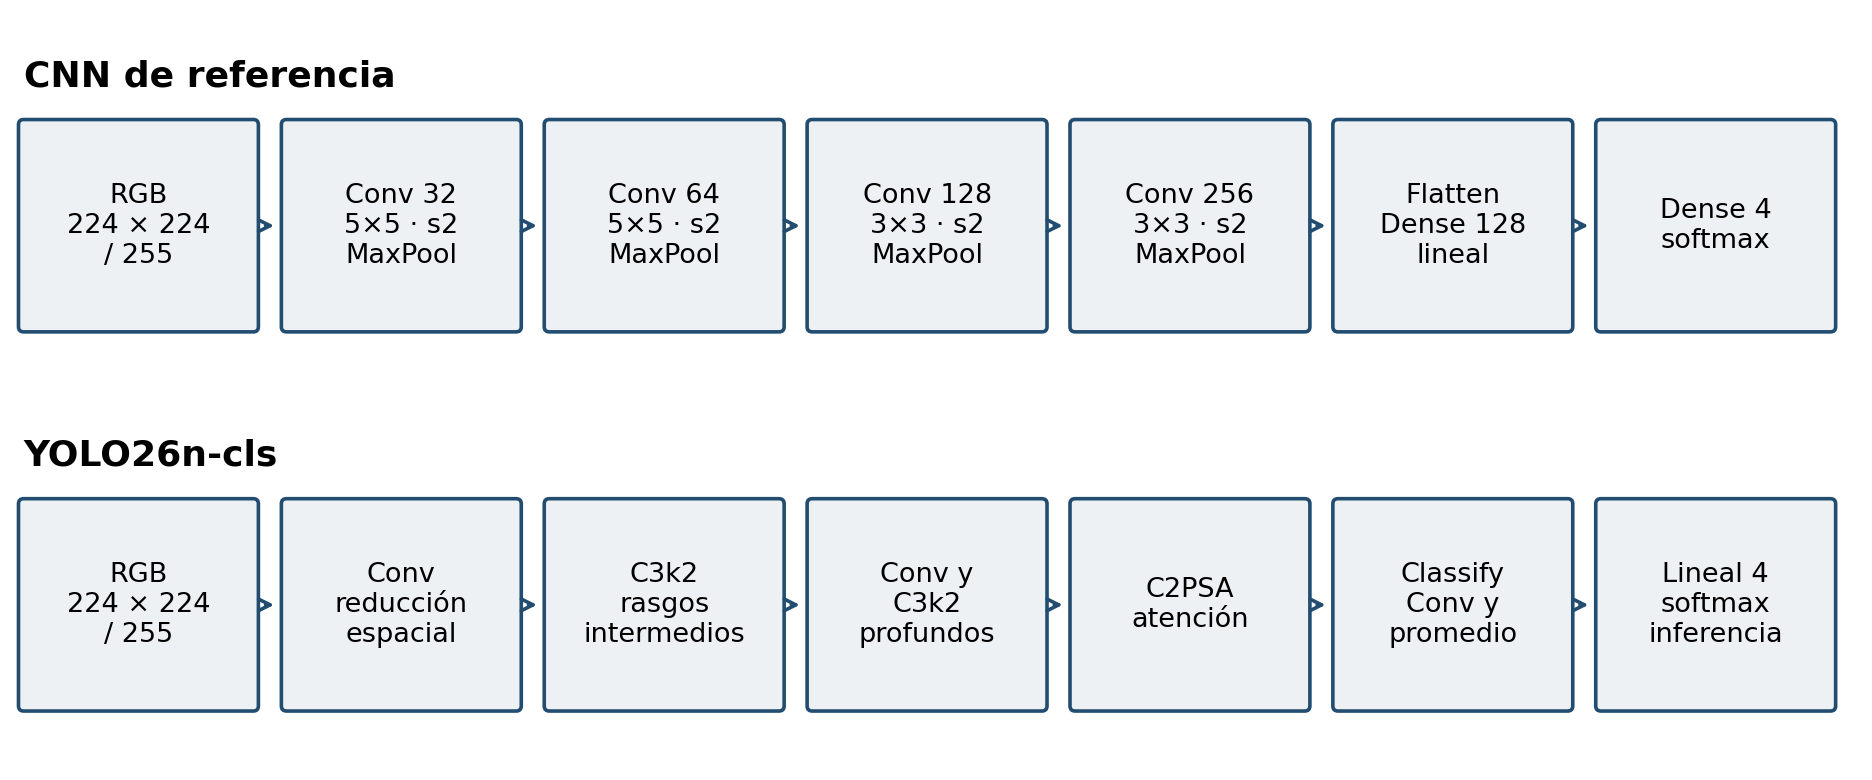
\includegraphics[width=\textwidth]{architectures.png}
\caption{Esquemas de las arquitecturas usadas con cuatro salidas.}\label{fig:architectures}
\end{figure*}
La Fig.~\ref{fig:architectures} resume los recorridos desde los píxeles hasta las probabilidades. Las dos redes contienen convoluciones y difieren en sus bloques y cabeza de clasificación.
\subsection{Entrenamiento y ejecuciones repetidas}
Se usaron las semillas 17, 27, 37, 47 y 57 para cada arquitectura. La partición se mantuvo fija y la semilla de cada corrida controló inicialización y orden de entrenamiento. Cada ejecución se inició en un proceso independiente para liberar memoria y estado del framework al terminar. Las corridas finalizadas se identificaron mediante archivos de configuración y se conservaron al reanudar el trabajo. Una interrupción dentro de una corrida provoca su reinicio desde la misma semilla.

La Tabla~\ref{tab:hyper} resume el protocolo. Adam \cite{adam} tuvo tasa constante de 0,001 y épsilon de $10^{-7}$. Las redes recibieron lotes de 32 e imágenes RGB de 224 por 224. Se limitaron a 20 épocas con paciencia de cinco épocas sin mejora del F1 macro de validación. Se guardó el primer checkpoint que alcanzó cada máximo nuevo. La regla de parada y el conjunto de validación fueron comunes a ambas redes.

Los aumentos de entrenamiento se generaron con Pillow, con volteos horizontal y vertical independientes de probabilidad 0,5, y rotación uniforme entre -108 y 108 grados con interpolación bilineal y relleno negro. Se usó el mismo generador por semilla para ambos modelos. Estas transformaciones mantienen el diseño del notebook de referencia en cuanto a volteos y amplitud de rotación, con una implementación externa compartida. Su amplitud y el relleno pueden modificar la plausibilidad anatómica y constituyen una limitación del protocolo.

\begin{table}[t]
\caption{Hiperparámetros compartidos por ambas redes.}\label{tab:hyper}\centering
\begin{tabular}{ll}\toprule
Parámetro & Valor\\\midrule
Inicialización & Aleatoria\\
Optimizador & Adam\\
Tasa de aprendizaje & 0,001 constante\\
Épsilon & $10^{-7}$\\
Lote y tamaño & 32; RGB $224\times224$\\
Máximo de épocas & 20\\
Paciencia & 5 épocas\\
Selección & Mayor F1 macro de validación\\
Pérdida & Entropía cruzada multiclase\\
Semillas & 17, 27, 37, 47, 57\\\bottomrule
\end{tabular}
\end{table}
\subsection{Métricas, estadística y eficiencia}
El F1 macro es la media aritmética de los F1 de las cuatro clases, con igual contribución de cada categoría. Se calcularon además exactitud, precisión macro, recall macro y métricas individuales. Las clases sin predicciones positivas reciben cero en las divisiones indefinidas. Se guardaron probabilidades y etiquetas de cada imagen para que la matriz de confusión y los resúmenes puedan reconstruirse.

Las métricas de las cinco semillas se resumieron mediante media y desviación estándar muestral. Para la prueba bilateral se definieron cinco diferencias pareadas de F1, YOLO menos CNN, y se enumeraron las $2^5=32$ inversiones de signo. El valor p es la fracción de medias permutadas con magnitud al menos igual a la observada. Bajo la hipótesis nula, la validez del procedimiento requiere intercambiabilidad de signos de las diferencias. Esta hipótesis se refiere a la variabilidad de las corridas sobre la partición fija.

Con cinco pares, el menor valor p bilateral posible es 0,0625. Se reporta esta resolución junto con el efecto medio y cada diferencia. La prueba proporciona evidencia limitada con este tamaño muestral y la dependencia compartida del conjunto de prueba. Los resultados describen la variación del entrenamiento condicionada a una única partición. La incertidumbre debida a elegir otros pacientes o centros requeriría un diseño adicional.

El tiempo de entrenamiento se midió con reloj de pared desde el primer paso hasta guardar el último historial. Incluye aumentos, validación y escritura de checkpoints. Las descargas e instalaciones quedan fuera del intervalo. La latencia se midió con lote uno sobre imágenes ya decodificadas y redimensionadas. Se hicieron 20 pasos de calentamiento y 100 mediciones, incluyendo normalización, paso por la red y devolución de probabilidades a CPU. Se reportan mediana y percentil 95. Los tiempos describen el entorno de Colab asignado y las operaciones del protocolo, incluido el guardado de checkpoints. Su extrapolación a otro equipo requiere repetir la medición.

\section{Resultados}
\subsection{Desempeño en el conjunto de prueba}

El hardware registrado para las corridas fue Tesla T4. Los frameworks y sus versiones se registraron por ejecución junto con la plataforma y la versión de Python.

Se completaron diez entrenamientos y se evaluaron sus checkpoints seleccionados sobre las mismas 2.633 imágenes de prueba. Cada evaluación produjo probabilidades, etiquetas, métricas por clase y una matriz de confusión. La Tabla~\ref{tab:results} presenta la media y desviación estándar muestral de las cinco semillas. Los valores individuales se conservan en el consolidado y en los CSV por corrida.

\begin{table}[t]\caption{Resultados de prueba sobre cinco semillas.}\label{tab:results}\centering\begin{tabular}{lll}\toprule Métrica & CNN & YOLO26n-cls\\\midrule

F1 macro & 0{,}7077 $\pm$ 0{,}0234 & 0{,}7478 $\pm$ 0{,}0537\\

Exactitud & 0{,}7322 $\pm$ 0{,}0266 & 0{,}7676 $\pm$ 0{,}0538\\

Precisión macro & 0{,}7279 $\pm$ 0{,}0166 & 0{,}7685 $\pm$ 0{,}0496\\

Recall macro & 0{,}7160 $\pm$ 0{,}0212 & 0{,}7534 $\pm$ 0{,}0509\\

\bottomrule\end{tabular}\end{table}

YOLO26n-cls obtuvo el mayor F1 macro medio bajo este protocolo. La diferencia media YOLO menos CNN fue 0{,}0400. El valor p bilateral fue 0{,}1875. Con cinco diferencias pareadas, la resolución mínima de la prueba es 0{,}0625, por lo que este diseño carece de resolución para alcanzar el umbral convencional de 0{,}05 mediante esta prueba exacta.

\begin{figure}[t]\centering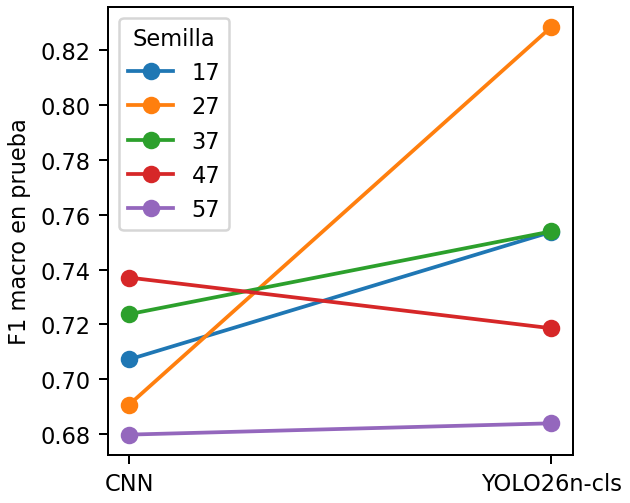
\includegraphics[width=\columnwidth]{paired_f1.png}\caption{F1 macro de prueba por semilla. Cada segmento conecta las corridas de la misma semilla.}\label{fig:paired}\end{figure}

La Fig.~\ref{fig:paired} permite examinar si la diferencia entre arquitecturas es consistente entre semillas y cómo se compara con la dispersión de cada modelo. Cada pareja usa la misma semilla y la misma secuencia de aumentos durante las épocas compartidas. Las arquitecturas consumen secuencias distintas al inicializar sus parámetros. La variabilidad entre semillas se refiere al entrenamiento y conserva fija la muestra de prueba.

\subsection{Comportamiento de aprendizaje}

\begin{figure*}[t]\centering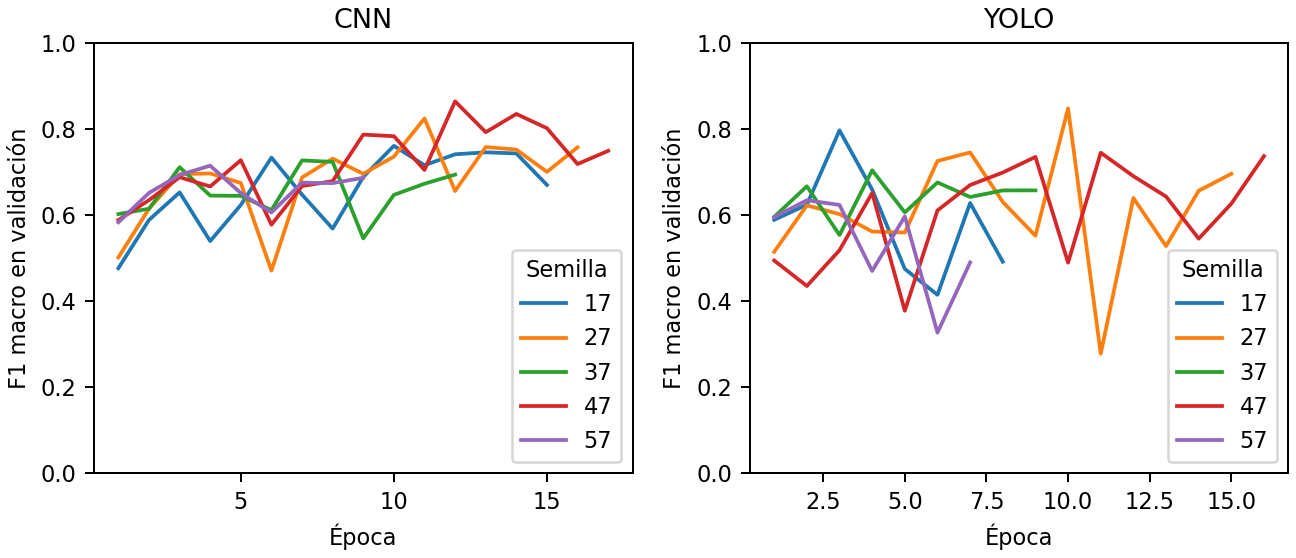
\includegraphics[width=\textwidth]{learning_curves.png}\caption{F1 macro de validación durante los cinco entrenamientos por arquitectura.}\label{fig:learning}\end{figure*}

\begin{figure*}[t]\centering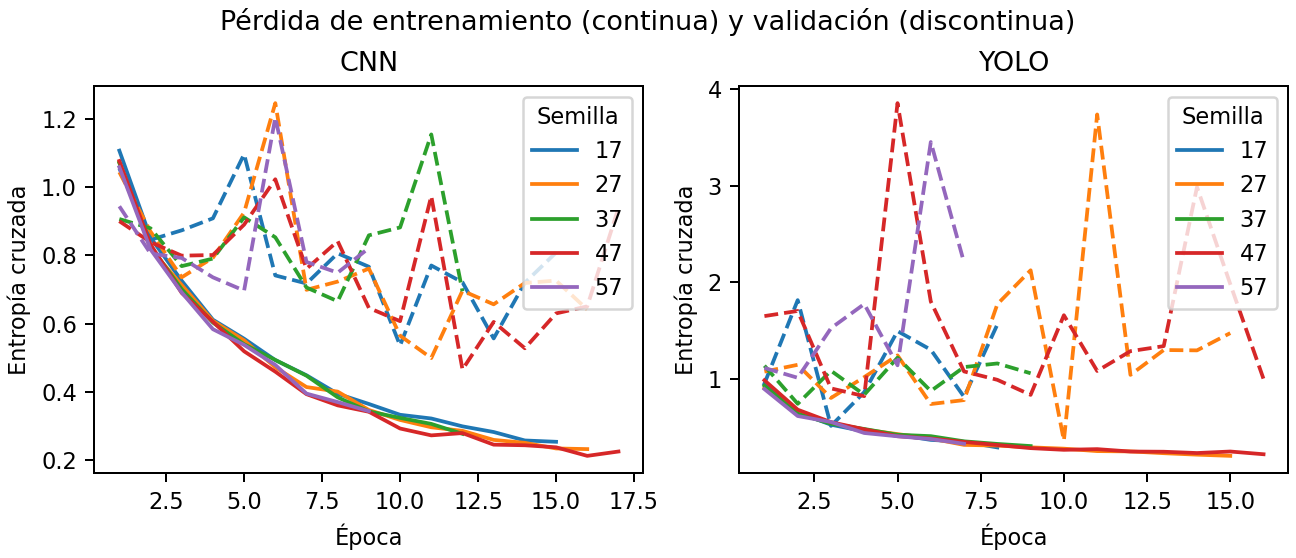
\includegraphics[width=\textwidth]{loss_curves.png}\caption{Pérdidas de entrenamiento y validación por época y semilla.}\label{fig:loss}\end{figure*}

Las Figs.~\ref{fig:learning} y~\ref{fig:loss} muestran la evolución de las corridas hasta la parada. Se comparan las curvas de validación con la reducción de pérdida de entrenamiento para identificar oscilaciones y posibles diferencias de generalización. El criterio común seleccionó el checkpoint por F1 macro de validación. Una reducción adicional de la pérdida de entrenamiento después del máximo de F1 puede coexistir con una degradación de la validación.

En CNN, el F1 macro medio de validación de los checkpoints seleccionados fue 0{,}7776 y el de la última época fue 0{,}7109. Esta comparación describe la evolución de validación y respalda conservar el checkpoint seleccionado antes de evaluar prueba.

En CNN, las épocas finales de las cinco semillas fueron 15, 16, 12, 17, 9. Los checkpoints seleccionados correspondieron a las épocas 10, 11, 7, 12, 4, respectivamente. La elección conserva el presupuesto máximo compartido y permite que la parada temprana determine duraciones distintas según la trayectoria de validación.

En YOLO26n-cls, el F1 macro medio de validación de los checkpoints seleccionados fue 0{,}7450 y el de la última época fue 0{,}6139. Esta comparación describe la evolución de validación y respalda conservar el checkpoint seleccionado antes de evaluar prueba.

En YOLO26n-cls, las épocas finales de las cinco semillas fueron 8, 15, 9, 16, 7. Los checkpoints seleccionados correspondieron a las épocas 3, 10, 4, 11, 2, respectivamente. La elección conserva el presupuesto máximo compartido y permite que la parada temprana determine duraciones distintas según la trayectoria de validación.

\subsection{Eficiencia computacional}

\begin{table}[t]\caption{Costo computacional de las cinco corridas.}\label{tab:time}\centering\begin{tabular}{lll}\toprule Medida & CNN & YOLO26n-cls\\\midrule

Entrenamiento (s) & 359{,}4227 $\pm$ 84{,}8609 & 350{,}1515 $\pm$ 131{,}8539\\

Latencia p50 (ms) & 1{,}5233 $\pm$ 0{,}2536 & 6{,}3146 $\pm$ 0{,}1105\\

Latencia p95 (ms) & 2{,}2994 $\pm$ 0{,}6333 & 8{,}0960 $\pm$ 1{,}1326\\

\bottomrule\end{tabular}\end{table}

La Tabla~\ref{tab:time} muestra el costo observado. CNN presentó la menor latencia mediana media bajo el protocolo de lote uno. Estos tiempos incluyen los pasos de inferencia definidos en métodos y dependen del hardware, el framework y las condiciones de carga. El tiempo total de entrenamiento también depende de cuántas épocas completó cada corrida. Se conservaron ambas medidas para diferenciar costo por predicción y costo de aprendizaje.

\begin{figure}[t]\centering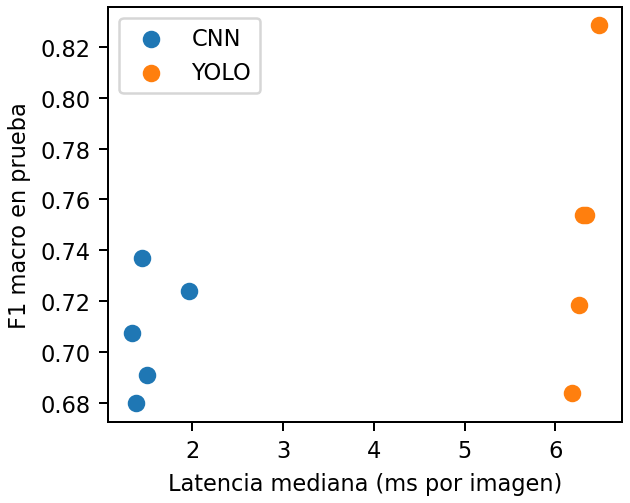
\includegraphics[width=\columnwidth]{f1_latency.png}\caption{F1 macro frente a latencia mediana de inferencia. Cada punto corresponde a una semilla.}\label{fig:latency}\end{figure}

La Fig.~\ref{fig:latency} combina las métricas predictiva y computacional para examinar compromisos entre exactitud y tiempo. La nube de puntos informa sobre la dispersión observada bajo la misma partición. La comparación no incluye compilación a ONNX o TensorRT, y cualquier extensión a otros equipos requiere repetir la medición con el mismo protocolo.

\subsection{Errores por clase y mapas de activación}

\begin{table}[t]\caption{Métricas medias por clase en prueba.}\label{tab:class}\centering\begin{tabular}{llrrr}\toprule Modelo & Clase & P & R & F1\\\midrule

CNN & cyst & 0{,}7310 & 0{,}9034 & 0{,}8077\\

CNN & normal & 0{,}7310 & 0{,}7393 & 0{,}7235\\

CNN & stone & 0{,}5955 & 0{,}4389 & 0{,}4858\\

CNN & tumor & 0{,}8540 & 0{,}7826 & 0{,}8140\\

YOLO26n-cls & cyst & 0{,}7375 & 0{,}9666 & 0{,}8347\\

YOLO26n-cls & normal & 0{,}7660 & 0{,}7306 & 0{,}7436\\

YOLO26n-cls & stone & 0{,}7074 & 0{,}5028 & 0{,}5843\\

YOLO26n-cls & tumor & 0{,}8630 & 0{,}8136 & 0{,}8284\\

\bottomrule\end{tabular}\end{table}

La Tabla~\ref{tab:class} permite evaluar el aporte de cada clase al promedio macro. Sus precisiones y recalls se interpretan junto con las matrices de confusión para distinguir falsos positivos y falsos negativos. Las diferencias entre clases pueden reflejar apariencia, tamaño de muestra, mezcla de modalidades o calidad de las etiquetas. El experimento carece de metadatos suficientes para atribuirlas a una sola causa.

\begin{figure}[t]\centering\includegraphics[width=\columnwidth]{cnn-17/confusion.png}\caption{Matriz de confusión de CNN, semilla 17. Filas con etiqueta real y columnas con predicción.}\label{fig:conf-cnn}\end{figure}

En la corrida ilustrativa de CNN con semilla 17, la confusión dirigida más frecuente fue stone como normal, con 169 imágenes. La Fig.~\ref{fig:conf-cnn} muestra todos los conteos. Esta semilla se fijó para las figuras ilustrativas antes de consultar la prueba y el resumen principal incluye las cinco corridas.

\begin{figure}[t]\centering\includegraphics[width=\columnwidth]{yolo-17/confusion.png}\caption{Matriz de confusión de YOLO26n-cls, semilla 17. Filas con etiqueta real y columnas con predicción.}\label{fig:conf-yolo}\end{figure}

En la corrida ilustrativa de YOLO26n-cls con semilla 17, la confusión dirigida más frecuente fue stone como cyst, con 151 imágenes. La Fig.~\ref{fig:conf-yolo} muestra todos los conteos. Esta semilla se fijó para las figuras ilustrativas antes de consultar la prueba y el resumen principal incluye las cinco corridas.

\begin{figure}[t]\centering\includegraphics[width=\columnwidth]{cnn-17/gradcam.png}\caption{Grad-CAM de la CNN, semilla 17, en la tercera convolución. El mapa se calcula respecto a la clase predicha.}\label{fig:gradcam}\end{figure}

El mapa Grad-CAM \cite{gradcam} de la Fig.~\ref{fig:gradcam} usa el gradiente de la clase predicha sobre la tercera convolución. Esta capa conserva una cuadrícula espacial de 7 por 7, mientras que la cuarta alcanza una resolución muy reducida. El mapa ofrece una localización gruesa de las activaciones relacionadas con la salida. La selección de la imagen sigue la regla de error de mayor confianza de la semilla 17, o la primera imagen si esa corrida carece de errores. El mapa requiere lectura junto con la imagen, su etiqueta y su predicción.


En promedio, Stone obtuvo el menor F1 de las cuatro clases: 0{,}4858 en la CNN y 0{,}5843 en YOLO26n-cls. Su recall medio fue 0{,}4389 y 0{,}5028, respectivamente. Este resultado identifica una dificultad persistente que el promedio global puede ocultar. Las cifras corresponden a las etiquetas del conjunto y deben interpretarse junto con su procedencia heterogénea.

El ejemplo de la Fig.~\ref{fig:gradcam}, \texttt{kidney-stone-0066.jpg}, está etiquetado como Stone y fue clasificado como Cyst con puntuación softmax de 0{,}9998. El mapa resalta bandas curvas periféricas del tercio inferior. Esta distribución permite plantear una revisión de posibles atajos visuales asociados al encuadre. El mapa, por sí solo, no demuestra la causa del error ni valida una localización anatómica. Las salidas softmax de este estudio no fueron calibradas.

\section{Discusión}
Los resultados caracterizan un protocolo con presupuesto compartido, inicialización aleatoria y una partición congelada. El número de parámetros y el diseño de la representación producen costos distintos, pero su relación con el F1 depende del entrenamiento observado. La pérdida, el F1 de validación y las predicciones de prueba permiten estudiar estas diferencias sin usar prueba para seleccionar hiperparámetros.

El resultado histórico del notebook de referencia se obtuvo con otra división y seleccionando por exactitud de validación. La retirada de duplicados y el agrupamiento de imágenes similares modifican la dificultad y el tamaño de las muestras. Por ello, el contraste con esa cifra exige considerar esas diferencias. El valor de la reproducción está en conservar la arquitectura y hacer trazables los cambios de protocolo.

La ausencia de identificadores de paciente es una limitación central. Un agrupamiento visual puede reducir fugas detectables y aun así dejar cortes relacionados en conjuntos distintos. La heterogeneidad de fuentes agrega otra incertidumbre. El formato y los rasgos de adquisición pueden estar asociados con las etiquetas, y los mapas de activación ofrecen una comprobación exploratoria que requiere una validación clínica y por fuente más detallada.

La validación reúne 526 imágenes y se consulta al final de cada época. Su tamaño y el agrupamiento visual pueden contribuir a oscilaciones del F1 y a cambios del checkpoint elegido. Las curvas se conservan para examinar esta sensibilidad. La comparación final mantiene el conjunto de prueba reservado durante todas esas decisiones.

El uso de cinco semillas permite cuantificar variación debida al entrenamiento, pero conserva el mismo conjunto de prueba. La prueba exacta bilateral tiene resolución limitada y requiere su hipótesis de intercambiabilidad de signos. La magnitud del efecto y las diferencias individuales aportan información adicional. La variabilidad entre centros y pacientes requeriría particiones por paciente verificables y validación externa.

El entrenamiento desde cero alinea la condición de partida. La receta de Adam compartida facilita comparar las arquitecturas bajo un mismo esquema, aunque no optimiza por separado la receta de cada red. Un estudio posterior podría comparar transferencia en ambas arquitecturas y establecer un presupuesto de búsqueda equivalente. Esas variantes requieren nuevos experimentos y un conjunto de prueba reservado para su evaluación.

Los giros amplios, volteos y relleno negro reproducen la intención de aumentos de la referencia con una implementación común. Pueden producir vistas de plausibilidad anatómica limitada. Un análisis adicional podría estudiar su efecto mediante validación y fijar una configuración alternativa antes de evaluar un nuevo conjunto de prueba. El protocolo actual permite atribuir sus resultados a decisiones específicas que están registradas en código.

La latencia se midió con entradas preparadas y lote uno. Un sistema que lea imágenes desde disco, reciba estudios completos o aplique otros preprocesamientos tendría un costo adicional. Los tiempos registrados permiten comparar las implementaciones probadas y deben acompañarse de la identificación de hardware y software. La cifra de entrenamiento incluye validación y guardado, por lo que su interpretación considera tanto las épocas completadas como la velocidad de cada paso.

\balance
\section{Conclusiones}
Se compararon una CNN de referencia y YOLO26n-cls sobre una partición común de imágenes renales, con cinco semillas por arquitectura. La auditoría identificó 1.225 copias exactas adicionales y permitió conservar 10.531 imágenes con agrupamiento de similitud antes de la partición. YOLO26n-cls obtuvo el mayor F1 macro medio en el experimento, mientras que CNN presentó la menor latencia mediana media. El efecto medio YOLO menos CNN fue 0{,}0400 y el valor p bilateral exacto fue 0{,}1875.

La elección práctica debe considerar el F1 de cada clase, la dispersión entre corridas y el costo por imagen. La resolución estadística de cinco pares y la ausencia de identificadores verificables de paciente limitan la fuerza de las conclusiones. Como trabajo futuro se plantea recuperar procedencia y agrupación clínica, realizar validación externa y estudiar configuraciones de transferencia con presupuesto equivalente. El repositorio local conserva manifiesto, código, configuraciones y predicciones para reproducir la comparación.
\subsection*{Uso de inteligencia artificial}
Se utilizó Codex como apoyo para la implementación, automatización del experimento y elaboración de la documentación. Las métricas se verificaron mediante los registros y predicciones guardadas. La revisión e interpretación final corresponden a los autores.
\clearpage
\begin{thebibliography}{99}
\bibitem{dataset}GonzaJL, ``Riñones - Cyst, Stone, Tumor, Normal - Dataset,'' Kaggle, ver. 2, 2023. [En línea]. Disponible: \url{https://www.kaggle.com/datasets/gonzajl/riones-cyst-stone-tumor-normal-dataset}
\bibitem{baseline}A. Tahmeed, ``Cyst, Stone, Tumor, Normal Classify,'' Kaggle notebook, consultado el 11 de noviembre de 2026. [En línea]. Disponible: \url{https://www.kaggle.com/code/ahnaftahmeed/cyst-stone-tumor-normal-classify}
\bibitem{yolo}J. Redmon, S. Divvala, R. Girshick y A. Farhadi, ``You Only Look Once: Unified, Real-Time Object Detection,'' en \emph{Proc. IEEE CVPR}, 2016, pp. 779--788, doi: 10.1109/CVPR.2016.91.
\bibitem{yolo26}G. Jocher, J. Qiu, M. Liu, S. Lyu, F. C. Akyon y M. E. Kalfaoglu, ``Ultralytics YOLO26: Unified Real-Time End-to-End Vision Models,'' \emph{arXiv:2606.03748}, 2026. [En línea]. Disponible: \url{https://arxiv.org/abs/2606.03748}
\bibitem{ultralytics}Ultralytics, ``Image Classification with Ultralytics YOLO,'' documentación y código fuente, paquete ver. 8.4.0, 2026. [En línea]. Disponible: \url{https://docs.ultralytics.com/tasks/classify/} y \url{https://github.com/ultralytics/ultralytics/tree/v8.4.0}
\bibitem{islam}M. N. Islam, M. Hasan, M. K. Hossain, M. G. R. Alam, M. Z. Uddin y A. Soylu, ``Vision transformer and explainable transfer learning models for auto detection of kidney cyst, stone and tumor from CT-radiography,'' \emph{Scientific Reports}, vol. 12, art. 11440, 2022, doi: 10.1038/s41598-022-15634-4.
\bibitem{pande}S. D. Pande y R. Agarwal, ``Multi-Class Kidney Abnormalities Detecting Novel System Through Computed Tomography,'' \emph{IEEE Access}, 2024, doi: 10.1109/ACCESS.2024.3351181.
\bibitem{kidneynet}S. N. Almuayqil, S. Abd El-Ghany, A. A. Abd El-Aziz y M. Elmogy, ``KidneyNet: A Novel CNN-Based Technique for the Automated Diagnosis of Chronic Kidney Diseases from CT Scans,'' \emph{Electronics}, vol. 13, no. 24, art. 4981, 2024, doi: 10.3390/electronics13244981.
\bibitem{lite}H. Xie, T. Yao y J. Cao, ``LiteRenalNet: A lightweight dual-branch network with channel-spatial co-attention for interpretable kidney CT classification,'' \emph{Journal of King Saud University Computer and Information Sciences}, vol. 38, art. 814, 2026, doi: 10.1007/s44443-026-01223-2.
\bibitem{adam}D. P. Kingma y J. Ba, ``Adam: A Method for Stochastic Optimization,'' en \emph{Proc. ICLR}, 2015, arXiv:1412.6980.
\bibitem{gradcam}R. R. Selvaraju, M. Cogswell, A. Das, R. Vedantam, D. Parikh y D. Batra, ``Grad-CAM: Visual Explanations from Deep Networks via Gradient-based Localization,'' en \emph{Proc. IEEE ICCV}, 2017, pp. 618--626, doi: 10.1109/ICCV.2017.74.
\end{thebibliography}

\end{document}
